\section{Defense strategies and Risk mitigation}

\subsection{Overview of Defense Strategies}

In the context where malicious software (malware) is increasingly growing in sophistication and evasion capability, relying solely on a single security solution has become outdated and insufficient to withstand threats. Modern organizations are required to implement a ``Defense-in-Depth'' strategy – establishing a comprehensive multi-layered protection framework to address cybersecurity risks \cite{kim2018fundamentals}.

The core objectives of this defense strategy are built upon three main operational pillars:

\begin{itemize}
    \item \textbf{Prevention (Prevent):} Stop intrusion attempts from outside right at the first barriers.
    \item \textbf{Detection (Detect):} Early and accurate identification of attack signs or abnormal behaviors within the system.
    \item \textbf{Mitigation (Mitigate):} Isolate risks, minimize damage, and quickly restore operations when a security incident occurs.
\end{itemize}

To realize these three pillars, a complete defense strategy requires the coordinated integration of multiple protection layers. Among them, User Authentication plays the role of a foundational building block and the first line of defense, enabling access control, ensuring traceability, and protecting data integrity.

However, strong authentication is only the starting point. To make the system truly resilient against all attack scenarios, organizations must combine authentication with other risk management pillars, including: continuously reducing vulnerabilities through Patch Management, ensuring availability through Backup Strategy, proactively responding through Incident Response processes, and finally strengthening the weakest link through User Awareness enhancement. The combination of all these factors determines the survivability of a modern information system.

\subsection{Defense-in-Depth Model}

\subsubsection{Concept of Defense-in-Depth}

Defense-in-Depth is a cybersecurity strategy and architecture model designed based on the principle of establishing multiple independent and sequential protection layers. The core philosophy of this model is the acknowledgment that no single security control is perfect. By stacking multiple defense layers, if a malicious actor (malware) or hacker bypasses one layer, the subsequent layers will continue to operate to block, slow down the intrusion process, and protect system assets.

Typical technical defense layers in this model include:

\begin{itemize}
    \item \textbf{Network/Perimeter Layer:} Acts as the outermost defensive boundary, using Firewalls and Intrusion Detection/Prevention Systems (IDS/IPS) to control, filter, and monitor all incoming and outgoing network traffic.
    
    \item \textbf{Endpoint Layer:} Provides direct protection at user-facing devices (workstations, mobile devices, servers) through Antivirus software and Endpoint Detection and Response (EDR).
    
    \item \textbf{Application Layer:} Prevents exploitation of software vulnerabilities by applying Secure Coding practices from the development stage and using Web Application Firewalls (WAF).
    
    \item \textbf{Data Layer:} The most critical core layer, protecting data confidentiality through strong Encryption mechanisms and strict Access Control policies.
\end{itemize}

\subsubsection{Integration of the AAA Access Control Framework}

To ensure that defense layers from network to data operate consistently and tightly, organizations need to implement a unified control mechanism called the AAA framework (Authentication, Authorization, Accounting) \cite{ref2}.

The AAA framework governs the entire lifecycle of an entity’s access to the system:

\begin{itemize}
    \item \textbf{Authentication (Authentication - Identity Check):} This is the mandatory starting point of the AAA framework. It acts as a ``gatekeeper'', answering the question: ``Is this user or device truly the identity they claim to be?''. If this identity verification step is not passed, the subject will be denied access immediately at the outer layer and cannot proceed deeper into application or data layers.
    
    \item \textbf{Authorization (Authorization - Permissions):} After the system successfully verifies identity in the Authentication step, the Authorization process takes place. This step strictly applies the Principle of Least Privilege, meaning only granting users the minimum permissions necessary to perform their tasks.
    
    \item \textbf{Accounting (Accounting/Logs):} The final step is to monitor and record all user actions after login. All actions such as opening files, downloading, or modifying data are stored in system logs. This creates non-repudiation and serves as important data for incident investigation.
\end{itemize}

\subsection{Enhancing Access Control and User Authentication}

\subsubsection{Role of Authentication in Preventing Attacks}

User Authentication is the main defensive shield (main shield) against attackers attempting to take over system accounts. In the context of malware distribution campaigns often accompanied by credential theft, a strong authentication mechanism will neutralize the attacker’s ability to perform masquerade attacks on legitimate users, even if they have obtained part of the information.

\subsubsection{Weaknesses of Single-Factor Authentication (SFA) and Common Attack Methods}

Single-Factor Authentication (SFA), usually based only on passwords (``something you know''), is currently considered very weak and vulnerable. Attackers can easily bypass SFA through the following methods:

\begin{itemize}
    \item \textbf{Brute Force \& Dictionary Attacks:} Attackers use automated tools to try thousands of password combinations or use lists of commonly used/leaked passwords. The RockYou data breach (2009) with more than 32 million exposed passwords is evidence of the danger of weak password practices and password reuse.
    
    \item \textbf{Rainbow Table Attacks:} Exploit insecure password storage systems (hashed passwords without salting) to reverse back to the original passwords, typically the Adobe breach (2013) with 150 million compromised accounts.
\end{itemize}

\subsubsection{Levels of Upgrading Authentication Strategy}

To defend effectively, organizations must upgrade authentication systems based on the combination of multiple independent factors:

\begin{itemize}
    \item \textbf{Two-Factor Authentication (2FA) and Multi-Factor Authentication (MFA):} Require users to provide at least one additional verification factor beyond a password, such as ``Something you have'' (OTP via phone, hardware token) or ``Something you are'' (Biometrics: fingerprint, face).
\end{itemize}

\begin{figure}[h]
    \centering
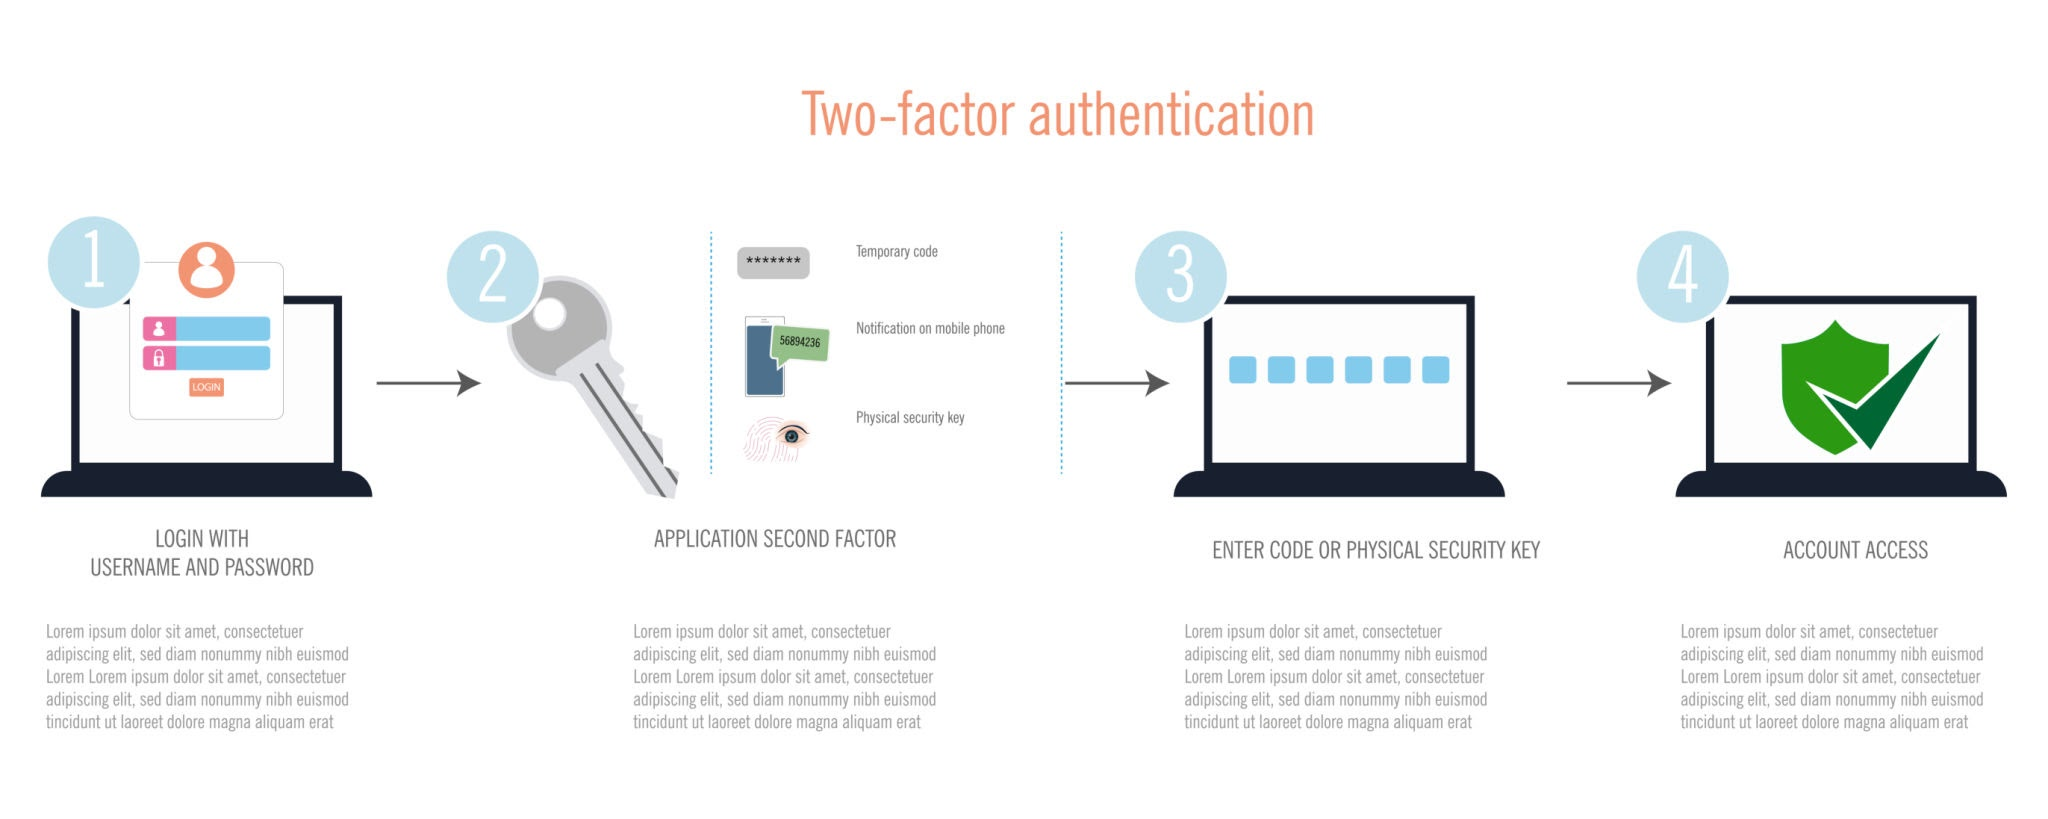
\includegraphics[width=0.8\textwidth]{images/mfa_report.png}
    \caption{Security reports indicate that implementing MFA can prevent more than 99\% of automated account takeover attacks \cite{ref3}.}
\end{figure}

\begin{itemize}
    \item \textbf{Passwordless Authentication (Passwordless \& Passkeys):} This is the most advanced defense technology trend today, based on WebAuthn and FIDO standards. Instead of sharing passwords (shared secrets), Passkeys use cryptographic key pairs stored directly on the device. This method not only optimizes user experience but also completely eliminates risks such as phishing-resistant attacks and credential stuffing \cite{ref4}.
\end{itemize}

\subsubsection{Real-world Case Study: Security Transformation at Google}

To cope with the massive scale of online fraud, Google implemented a historic authentication transformation strategy:

\begin{itemize}
    \item \textbf{Phase 1:} Mandatory application of MFA for high-risk accounts (such as administrators) and expansion to general users, combined with push-based authentication to improve usability.
    
    \item \textbf{Phase 2:} Pioneered global-scale Passkey deployment. This process helped Google significantly reduce operational costs (related to password reset support and account recovery) and protect billions of users from the most sophisticated phishing techniques.
\end{itemize}

\subsection{Patch Management Process and Risk Reduction}

\subsubsection{Concept and Importance of Patch Management}

Patch Management is not simply pressing the ``update'' button on software; it is a systematic strategic process aimed at fixing security vulnerabilities before they are exploited by attackers \cite{kim2018fundamentals}.

In information security, there exists a concept called the ``Vulnerability Window'' – this is the period from when a software vulnerability is disclosed until the system is actually patched to fix that vulnerability. Delays, postponement, or ignoring the update process are the root cause that create conditions for malware to spread and cause cyberattacks on a large scale.

\subsubsection{Standard Patch Management Process}

To ensure the system is not disrupted due to compatibility issues of new updates while still closing vulnerabilities, a professional patch management process in enterprises will go through the following steps:

\begin{itemize}
    \item \textbf{Discovery \& Assessment:} Continuously monitor security bulletins to detect new vulnerabilities. Evaluate the severity of vulnerabilities for the current system.
    
    \item \textbf{Testing:} Never deploy patches directly to the entire production system. Updates must be installed in a simulated environment (Sandbox/Test environment) to ensure they do not conflict with existing business applications.
    
    \item \textbf{Deployment:} Schedule official updates, prioritizing servers/devices storing important data first.
    
    \item \textbf{Verification \& Monitoring:} Re-check to ensure the patch has been successfully applied and the system operates stably.
\end{itemize}

\subsubsection{Real-world Case Study: WannaCry Ransomware Disaster}

The WannaCry ransomware outbreak in May 2017 is the most valuable evidence of weaknesses in patch management processes of organizations worldwide \cite{ref5}.

\begin{itemize}
    \item \textbf{Vulnerability Context:} WannaCry malware was designed to automatically spread through internal networks by exploiting a critical vulnerability in the Windows SMB protocol (identifier CVE-2017-0144, also known as EternalBlue).
    
    \item \textbf{Deadly Delay:} In fact, Microsoft released a patch for this vulnerability in March 2017. However, many government agencies, hospitals, and large corporations did not perform updates in time.
    
    \item \textbf{Consequences:} More than 200,000 computers in over 150 countries were infected, all data was encrypted and ransom demanded, paralyzing healthcare and transportation systems in many countries. If the patch management process had been strictly implemented immediately when Microsoft released the update, this entire disaster could have been completely prevented from the beginning.
\end{itemize}

\subsection{Data Backup Strategy and the 3-2-1 Rule}

\subsubsection{Importance of Backup in Security}

Data backup is considered the ``last survival shield'' when outer technical defense layers fail before disasters, especially destructive attacks from ransomware. Considering under the core security model CIA Triad (CIA Triad), backup strategy plays a decisive role in protecting Availability, ensuring systems and business services can operate again in the shortest time after incidents.

\subsubsection{Gold Standard: The 3-2-1 Backup Rule}

To ensure the highest resilience against data loss risks, organizations are recommended to strictly follow the 3-2-1 rule:

\begin{itemize}
    \item \textbf{3 copies of data:} Always maintain at least three copies of important data (including 1 original copy in operation and 2 independent backup copies). Having multiple copies helps minimize the risk of total loss if one copy is corrupted or infected.
    
    \item \textbf{2 different storage media types:} Store backup copies on at least two different physical technologies or storage systems (for example: NAS and tape). This helps avoid mass hardware failure risks.
    
    \item \textbf{1 offsite backup:} It is mandatory to have at least one backup located outside the main data center (for example: Cloud or another geographic location). This is the most important protection layer against physical disasters or large-scale malware spread.
\end{itemize}

\subsubsection{Enhanced Defense: Immutable and Air-gapped Backup}

In the context of increasingly sophisticated ransomware, they not only encrypt original data but also attempt to delete backup copies connected to the system. Therefore, backup strategies must be upgraded with the following technologies:

\begin{itemize}
    \item \textbf{Immutable Backup:} Data is stored using the WORM (Write Once, Read Many) mechanism, cannot be modified or deleted within a defined period, even by administrators.
    
    \item \textbf{Air-gap:} Backup copies are completely isolated from internal networks and the Internet, only temporarily connected during backup execution.
\end{itemize}

\subsubsection{Core Benefits and Practical Application}

Implementing a proper backup strategy brings essential benefits:

\begin{itemize}
    \item Fast and accurate data recovery.
    \item Neutralizing pressure from ransomware attacks.
    \item Ensuring business continuity.
\end{itemize}

\textbf{Real-world example:} An enterprise is attacked by ransomware causing all data to be encrypted. Thanks to applying the 3-2-1 rule with backup copies on Cloud, the IT team isolated the system, restored data from a clean backup copy and brought the system back to operation within only a few hours without paying ransom.

\subsection{Incident Response Lifecycle}

\subsubsection{Importance of Incident Response}

No matter how well an organization deploys Defense-in-Depth architecture, the risk of intrusion always exists. When an incident occurs (for example: a server is infected with malware, an administrator account is stolen), time is the core factor. A standardized Incident Response (IR) process will help the organization move from a ``passive, panicked'' state to a ``proactive controlled'' state, with the goal: early detection of incidents, minimizing impact as much as possible, and restoring systems quickly.

\subsubsection{Six Phases of the Incident Response Lifecycle}

A complete incident response lifecycle includes six phases:

\begin{itemize}
    \item \textbf{Preparation:} Establish a CSIRT team, build response playbooks, deploy monitoring tools and ensure backup systems are operational.
    
    \item \textbf{Detection:} Use SIEM or log systems to detect abnormal signs (for example: multiple failed login attempts or sudden increase in encrypted traffic).
    
    \item \textbf{Containment:} Isolate infected devices, segment the network and lock suspicious accounts to prevent malware from spreading.
    
    \item \textbf{Eradication:} Remove malware, delete backdoors and patch exploited vulnerabilities.
    
    \item \textbf{Recovery:} Restore systems from clean backup copies and monitor to ensure no reinfection occurs.
    
    \item \textbf{Lesson Learned:} Analyze root causes and upgrade the system (for example: transition from SFA to MFA).
\end{itemize}

\subsubsection{Real-world Example (Ransomware Response Scenario)}

An employee is tricked into downloading malware from a phishing email:

\begin{itemize}
    \item The EDR system detects abnormal encryption processes (Detection).
    \item The computer is isolated from the internal network (Containment).
    \item The IT team removes malware and cleans the system (Eradication).
    \item Data is restored from Cloud backup (Recovery).
    \item The company organizes anti-phishing training and upgrades authentication (Lesson Learned).
\end{itemize}

\subsection{User Awareness and Security Recommendations}

\subsubsection{Humans: The Weakest Link}

In any information system, no matter how perfectly Defense-in-Depth architecture is designed, humans are always considered the ``weakest link'' in the security chain. Instead of directly attacking technical systems, attackers often use Social Engineering techniques to manipulate users \cite{ref1}.

\subsubsection{Common Risky Behaviors}

Common mistakes that users often make include:

\begin{itemize}
    \item \textbf{Phishing:} Clicking on fraudulent links leading to credential theft or malware installation.
    
    \item \textbf{Downloading Malicious Software:} Installing cracked software or from untrusted sources.
    
    \item \textbf{Weak Passwords:} Using easily guessable passwords or reusing passwords.
    
    \item \textbf{Ignoring Updates:} Not updating systems, creating vulnerabilities for hackers to exploit.
\end{itemize}

\subsubsection{Recommendations and Solutions}

\textbf{For End Users:}
\begin{itemize}
    \item Use strong passwords and enable MFA.
    \item Participate in periodic security awareness training.
\end{itemize}

\textbf{For Technical Departments:}
\begin{itemize}
    \item Deploy SIEM, EDR for monitoring.
    \item Apply Network Segmentation.
\end{itemize}

\subsection{Future Trends and Conclusion}

\subsubsection{Emerging Cybersecurity Threats}

Modern attack trends include:

\begin{itemize}
    \item \textbf{AI-powered Malware:} Using AI to create sophisticated malware and phishing.
    
    \item \textbf{Fileless \& Living-off-the-Land:} Attacks without files, using system tools such as PowerShell.
    
    \item \textbf{Ransomware 3.0 \& Supply Chain Attack:} Attacks through supply chains (example SolarWinds).
\end{itemize}

\subsubsection{Overall Conclusion}

Cybersecurity threats are increasingly sophisticated and dangerous. Protecting systems cannot rely on a single solution.

To ensure the three core elements of information security:

\begin{itemize}
    \item Confidentiality
    \item Integrity
    \item Availability
\end{itemize}

Organizations need to:

\begin{itemize}
    \item Deploy multi-layered defense (Defense-in-Depth)
    \item Upgrade authentication (MFA, Passkey)
    \item Build operational and incident response processes
    \item Enhance user awareness
\end{itemize}


